% Preamble
	\documentclass[11pt,a4paper,openany]{book}
	% Packages
	\usepackage[utf8]{inputenc}
	\usepackage[T1]{fontenc}
	\usepackage{amsmath}
	\usepackage{amssymb}
	\usepackage{graphicx}
	\usepackage[spanish]{babel}
	\usepackage{xcolor}
		\definecolor{Azul}{rgb}{0.17, 0.4, 0.69}
		\definecolor{charcoal}{rgb}{0.21, 0.27, 0.31}
	\usepackage{varioref}
	\usepackage[left= 2.54cm, right=2.54cm, top=2.54cm, bottom=2.54cm]{geometry}
	\usepackage{setspace}
	\usepackage{lipsum}
	\usepackage{caption}
	\usepackage{float}
	\usepackage{booktabs}
	\usepackage{multirow}
	\usepackage{hyperref}
	\usepackage{times} % Time New Roman
	\usepackage{listings} % Program code
	% Customize
		% Line spread 
		\linespread{1.5}
		% Path for images
		\graphicspath{{Images/}}
		% Table 
		\captionsetup[table]{
			name = Tabla,
			labelsep = newline,
			justification = raggedright,
			singlelinecheck = false,
			labelfont = bf
		}
		% Program code
		\definecolor{codegreen}{rgb}{0,0.6,0}
		\definecolor{codegray}{rgb}{0.5,0.5,0.5}
		\definecolor{codepurple}{rgb}{0.58,0,0.82}
		\definecolor{backcolour}{rgb}{0.95,0.95,0.92}
		\lstdefinestyle{mystyle}{
			backgroundcolor=\color{backcolour},   
			commentstyle=\color{codegreen},
			keywordstyle=\color{magenta},
			numberstyle=\tiny\color{codegray},
			stringstyle=\color{codepurple},
			identifierstyle=\color{blue},
			basicstyle=\ttfamily\footnotesize,
			breakatwhitespace=false,         
			breaklines=true,                 
			captionpos=b,                    
			keepspaces=true,
			numbers=left,                    
			numbersep=5pt,                  
			showspaces=false,                
			showstringspaces=false,
			showtabs=false,                  
			tabsize=2
		}
		\lstset{style=mystyle}
% Document
	\begin{document}
		% FrontMatter
		% Beginning ----------------------------------------------
			\frontmatter
			% Cover
				% Titlepage
	\begin{titlepage}
		\begin{center}
			{\LARGE \textbf{Universidad Nacional Mayor de San Marcos}}\\
			\vspace{0.25cm}
			{\LARGE Universidad del Perú, Decana de América}\\
			\vspace{0.25cm}
			{\LARGE \textbf{Facultad de Ingeniería de Sistemas e Informática}}\\
			\vspace{0.5cm}
			{\LARGE Centro de Responsabilidad Social y Extensión Universitaria}\\
			\vspace{0.5cm}
			\begin{figure}[h]
				\centering
				\includegraphics[scale = 1]{LogoUNMSM2.png}
			\end{figure}
			\vspace{1cm}
			{\LARGE \textbf{Módulo I}}\\
			\vspace{0.5cm}
			\textcolor{charcoal}{\rule{150mm}{0.5mm}}
			\vspace{2mm}
				\begin{spacing}{1.5}
					{\LARGE PROYECTO DE BASE DE DATOS-RESTAURANTE}
				\end{spacing}
			\vspace{2mm}
			\textcolor{charcoal}{\rule{150mm}{0.5mm}}
			\vspace{0.7cm}\\
			{\Large \textbf{Jhon Roly Ordoñez Leon}}\\
			\vspace{5mm}
			{\Large Programa de Especialización en SQL Server}
			\vfill
			{\Huge \textbf{2022}}	
		\end{center}
	\end{titlepage}
			% Table of contents
				\tableofcontents
		% MainMatter
		% Center -------------------------------------------------	
			\mainmatter
			% Chapter 1: Descripción del proyecto
				% Chapter 1: Descripción del proyecto
	\chapter{Descripción del proyecto} \label{Cap: Descripción del proyecto}
	\begin{flushleft}
		\textbf{Misión} \\
		Satisfacer las expectativas de nuestros clientes
		y lograr que tenga una experiencia memorable.
	\end{flushleft}
	\begin{flushleft}
		\textbf{Visión} \\
		Ser destacado como el mejor restaurante en la localidad por nuestra gastronómia, atención y ambiente muy peculiar.
	\end{flushleft}
	\begin{flushleft}
		\textbf{Valores} \\
		\begin{itemize}
			\item Respeto
			\item Cortesía
			\item Honestidad
			\item Solidaridad
		\end{itemize}
	\end{flushleft}
	\textbf{Descripción del restaurante}\\
	El restautante es de alta cocina o también denominado \textit{Gourmet}. Es decir, los alimentos son de gran calidad y se sirven a la mesa. El pedido es “a la carta” o se elige de un “menú”, por lo que los alimentos se cocinan al momento. El costo depende del servicio y de la calidad de los platos que se consumen. Existen meseros, dirigidos por un Maitre. El servicio, la decoración, la ambientación, la comida y las bebidas se escogen cuidadosamente.

			% Chapter 2: Diagrama Entidad Relación (DER)
				% Chapter 2: Diagrama Entidad Relación (DER)
	\chapter{Diagrama Entidad Relación (DER)}\label{Chap: DER}
	A continuación se muestra el Diagrama Entidad Relación (DER) del proceso que sigue el restaurante.

	\begin{figure}[h!]
		\centering
		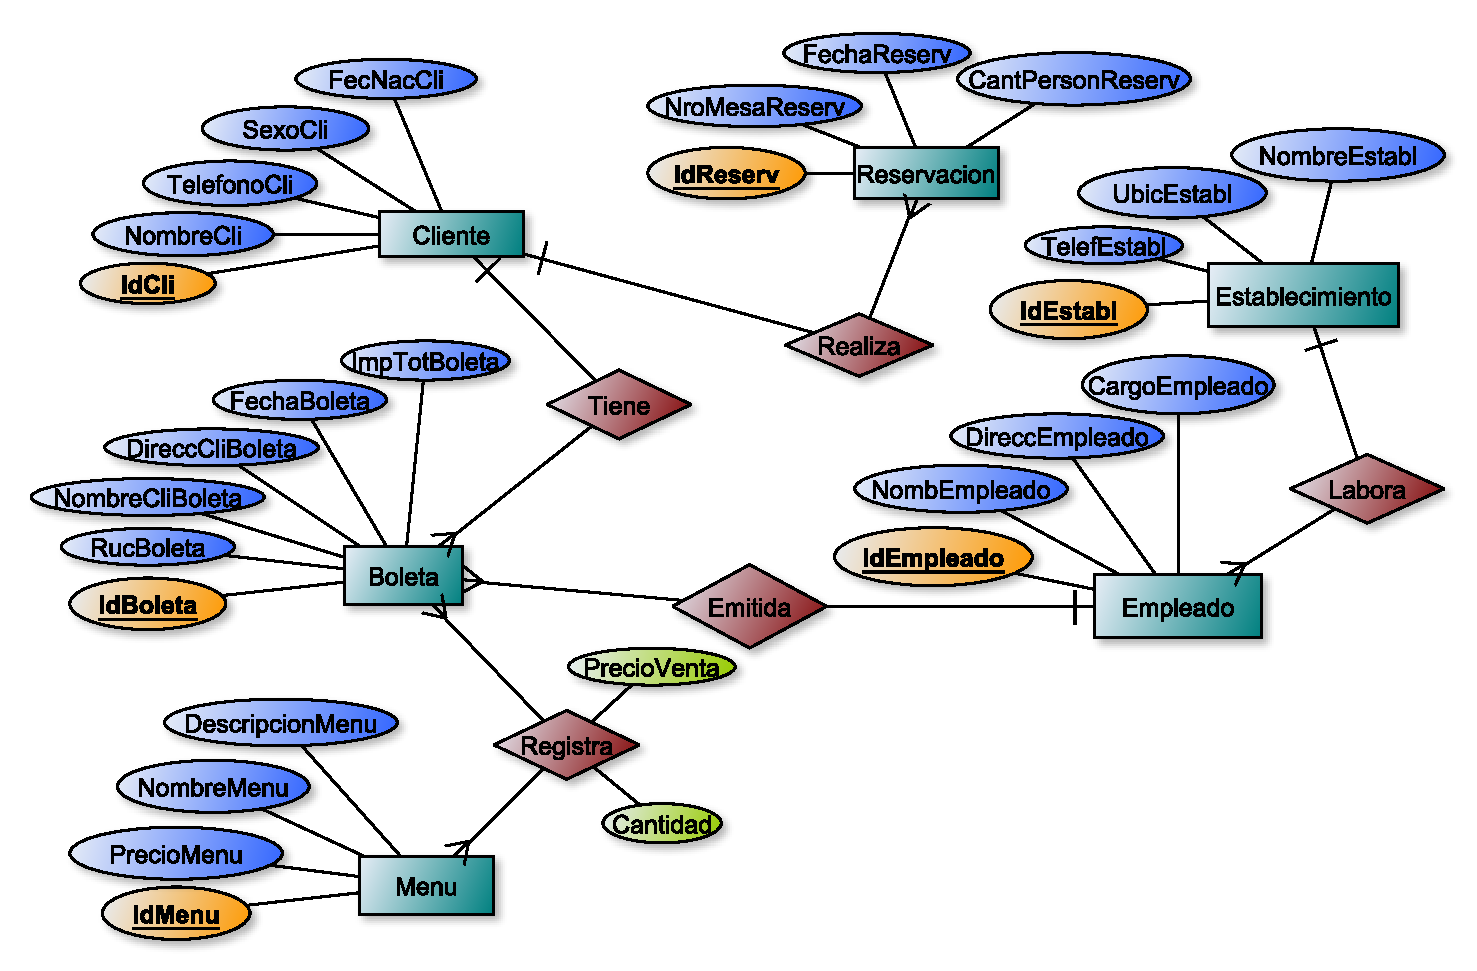
\includegraphics[scale = 0.6]{DER.pdf}
		\caption{Diagrama Entidad Relación (DER) de un Restaurante}
		\label{fig: DER Restaurante}
	\end{figure}
	
   La lectura del diagrama es lo siguiente: un cliente puede realizar muchas reservaciones y una reservación puede ser realizado solamente por un cliente; un cliente puede tener muchas boletas y una boleta le pertenece solamente a un cliente; una boleta puede ser emitido por un empleado y un empleado puede emitir muchas boletas; un empleado labora solamente en un establecimiento y en un establecimiento laboran muchos empleados; una boleta puede registrar muchos menús y un menú se puede registrar en muchas boletas.
	
	
	
	
	
			% Chapter 3: Programa SQL 
				% Chapter 3: Código de la consulta SQL 
	\chapter{Código de la consulta SQL}\label{Chap: Código de la consulta SQL}
	
	\lstinputlisting[language=SQL]{Code/CodeSQL.sql}
	 	
		
		
		
			% Chapter 4: Diagrama SQL
				% Chapter 4: Diagrama SQL
	\chapter{Diagrama de la base de datos}\label{Chap: Diagrama de la base de datos}
	A continuación se presenta el diagrama de la base de datos generado en SQL Server Managment Studio.
		\begin{figure}[h!]
			\centering
			\includegraphics[scale = 0.8]{DiagramSQL2.png}
			\caption{Diagrama de la base de datos}
			\label{fig: Diagrama de la base de datos}
		\end{figure}
	
	La lectura del diagrama de la base de datos es lo siguiente: un cliente puede realizar muchas reservaciones y una reservación puede ser realizado solamente por un cliente; un cliente puede tener muchas boletas y una boleta le pertenece solamente a un cliente; una boleta puede ser emitido por un empleado y un empleado puede emitir muchas boletas; un empleado labora solamente en un establecimiento y en un establecimiento laboran muchos empleados; una boleta puede registrar muchos menús y un menú se puede registrar en muchas boletas.	
		
		
		% BackMatter
	    % End ----------------------------------------------------
	    	\backmatter
	
			% Bibliography
			
			% Apendice
		
	\end{document}

